\documentclass[11pt, oneside]{article}   	% use "amsart" instead of "article" for AMSLaTeX format


% \usepackage{draftwatermark}
% \SetWatermarkText{Draft}
% \SetWatermarkScale{5}
% \SetWatermarkLightness {0.9} 
% \SetWatermarkColor[rgb]{0.7,0,0}


\usepackage{geometry}                		% See geometry.pdf to learn the layout options. There are lots.
\geometry{letterpaper}                   		% ... or a4paper or a5paper or ... 
%\geometry{landscape}                		% Activate for for rotated page geometryhttps://www.washingtonpost.com/world/europe/amid-impeachment-probe-gordon-sondland-is-overseeing-a-renovation-of-his-residence-that-has-cost-1-million-in-taxpayer-money/2019/10/16/d0eece92-ef86-11e9-bb7e-d2026ee0c199_story.html?tid=sm_tw
%\usepackage[parfill]{parskip}    		% Activate to begin paragraphs with an empty line rather than an indent
\usepackage{graphicx}				% Use pdf, png, jpg, or eps� with pdflatex; use eps in DVI mode
								% TeX will automatically convert eps --> pdf in pdflat						\label{thm:integral_domain}

								% TeX will automatically convert eps --> pdf in pdflatex		
\usepackage{amssymb}
\usepackage{amsmath}
\usepackage{amsthm}
\usepackage{mathrsfs}
\usepackage[hyphens,spaces,obeyspaces]{url}
\usepackage{url}
\usepackage{hyperref}
\usepackage{subcaption}
\usepackage{authblk}
\usepackage{mathtools}
\usepackage{graphicx}
\usepackage[export]{adjustbox}
\usepackage{fixltx2e}
\usepackage{hyperref}
\usepackage{alltt}
\usepackage{color}
\usepackage[utf8]{inputenc}
\usepackage[english]{babel}
\usepackage{float}
\usepackage{bigints}
\usepackage{braket}
\usepackage{siunitx}
\usepackage{mathtools}
\usepackage[most]{tcolorbox}




\usepackage[hyphenbreaks]{breakurl}

\newtheorem{thm}{Theorem}[section]
% \newtheorem{defn}[thm]{Definition}
\theoremstyle{definition}
\newtheorem{definition}{Definition}[section]
\newtheorem{proposition}{Proposition}[section]
\newtheorem{lemma}{Lemma}[section]
\newtheorem{example}{Example}[section]




\newcommand{\veq}{\mathrel{\rotatebox{90}{$=$}}}
\DeclareMathOperator{\bda}{\Big \downarrow}


\DeclareMathOperator{\E}{\mathbb{E}}
\newcommand{\argmax}{\operatornamewithlimits{argmax}}
\newcommand{\argmin}{\operatornamewithlimits{argmin}}

\title{Notes on Epicyclic Gearing}
\author{David Meyer \\ dmm@\{1-4-5.net,uoregon.edu\}}

\date{\today}							% Activate to display a given date or no date



\begin{document}
\maketitle

\section{Introduction}



\bigskip
\begin{center}
{\Large $\text{GR} = \frac{\text{Number of Teeth on the Driven Gear}}{\text{Number of Teeth on the Driver Gear}}$}
\end{center}


\begin{equation*}
\begin{array}{lllll}
  \text{One Metonic Cycle}
  &=& \text{19 tropical years}                     &\qquad  \mathrel{\#} \text {6,939.602 days}    \\
  &\approx& \text {235 synodic months}    &\qquad  \mathrel{\#} \text{6,939.688 days}      \\
  &\approx& \text {254 sidereal months}    &\qquad  \mathrel{\#} \text {6,939.702 days}     \\
  &\approx& \text {255 draconic months}   &\qquad  \mathrel{\#} \text {6,939.116 days}     \\
\end{array}
\end{equation*}



\bigskip
\bigskip
\begin{figure}[H]
 % \center{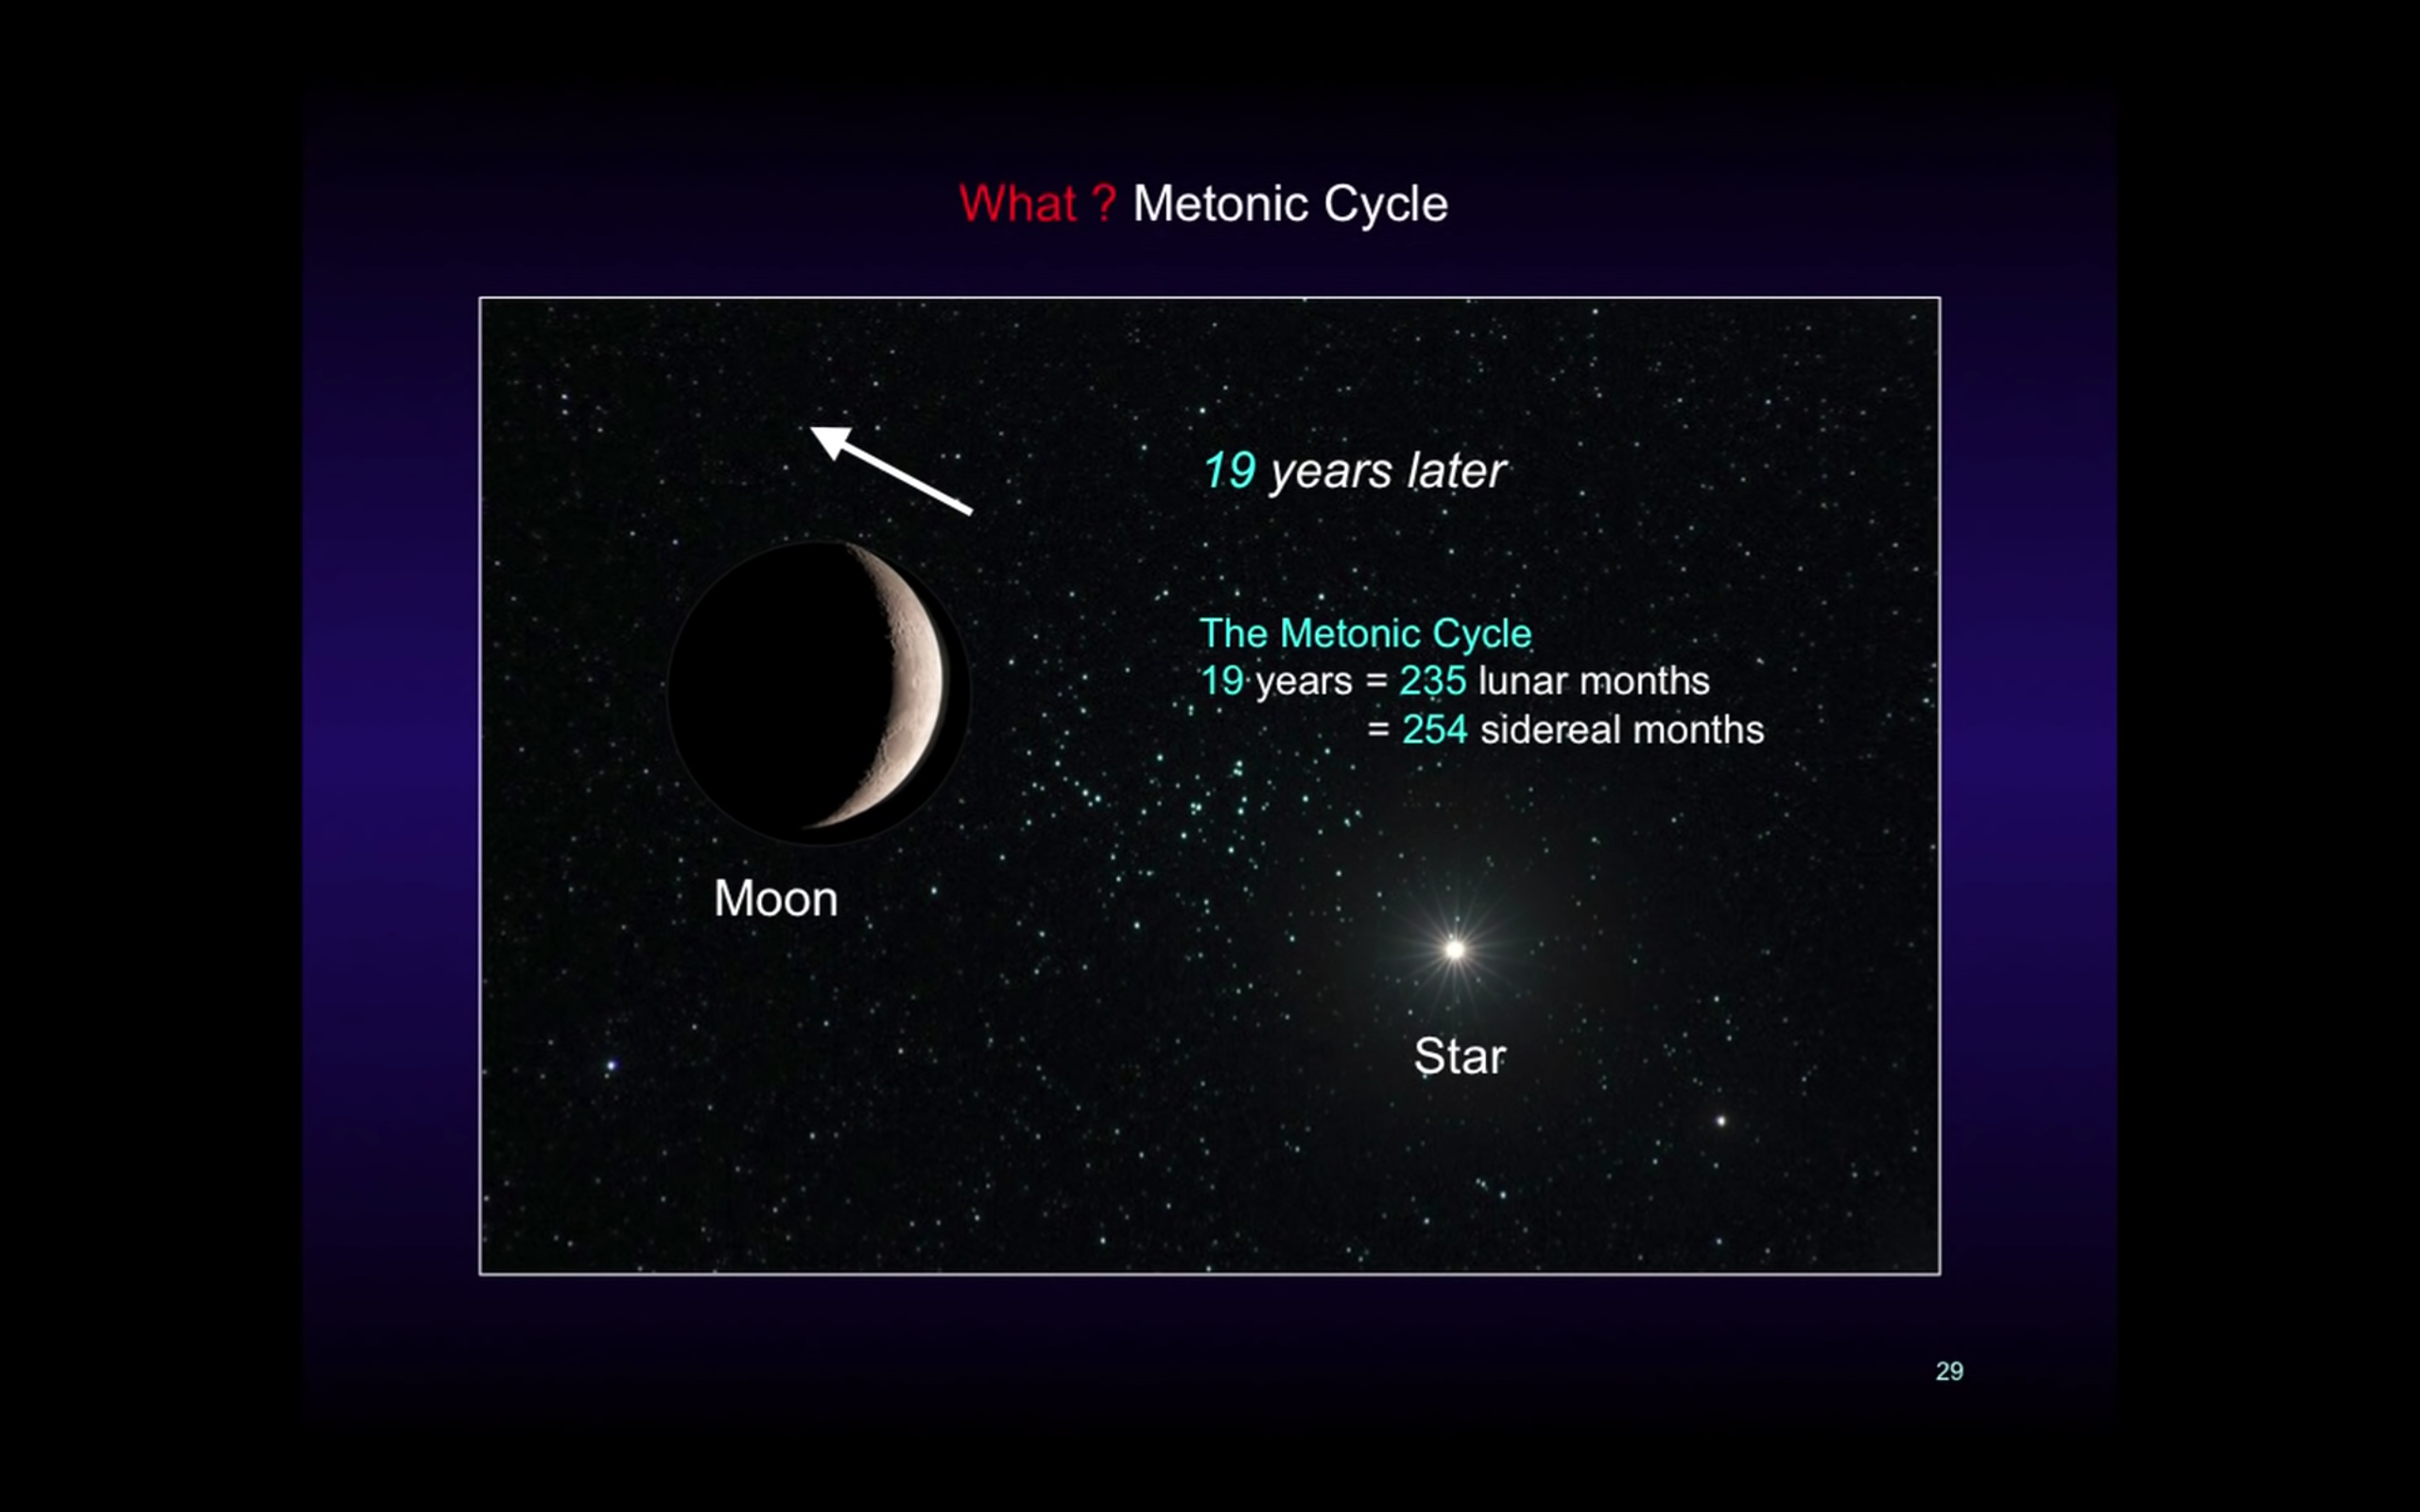
\includegraphics[scale=0.25,cfbox=red] {images/metonic.png}}
  \caption{The Metonic Cycle \cite{youtube:freeth2021}}
  \label{fig:metonic_cycle}
\end{figure}


\bigskip
\section{Acknowledgements}

\newpage
\bibliographystyle{plain}
\bibliography{/Users/dmm/papers/bib/astronomy}
\end{document} 
